% Template adapted from https://github.com/jgm/pandoc-templates/blob/master/default.latex
% To be used with XeLaTex in memoiR
%%%%%%%%%%%%%%%%%%%%%%%%%%%%%%%%%%%%%%%%%%%%%%%%%%%%%%%%%%%%%%%%%%%%%%%%%%%%%%%%%%%%%%%%%

% Options for packages loaded elsewhere
\PassOptionsToPackage{unicode=true}{hyperref}
\PassOptionsToPackage{hyphens}{url}
\PassOptionsToPackage{dvipsnames,svgnames*,x11names*}{xcolor}
% Right to left support


\documentclass[
  10pt,
  italian,
  a4paper,
  extrafontsizes,onecolumn,openright
  ]{memoir}

% Double (or whatever) spacing

% Math
\usepackage{amssymb, amsmath}
% mathspec: arbitrary math fonts
\usepackage{unicode-math}
\defaultfontfeatures{Scale=MatchLowercase}
\defaultfontfeatures[\rmfamily]{Ligatures=TeX,Scale=1}

% Fonts
% \usepackage{lmodern}
\usepackage{fontspec}

% Main font
% Specific sanserif font
% Specific monotype font
\setmonofont[Scale=0.75]{Operator Mono SSm Book}
% Specific math font
% Chinese, Japanese, Corean fonts

% Use upquote for straight quotes in verbatim environments
\usepackage{upquote}
% Use microtype
\usepackage[]{microtype}
\UseMicrotypeSet[protrusion]{basicmath} % disable protrusion for tt fonts

% Verbatim in note

% Color links
\usepackage{xcolor}

% Strikeout

% Necessary for code chunks
\usepackage{color}
\usepackage{fancyvrb}
\newcommand{\VerbBar}{|}
\newcommand{\VERB}{\Verb[commandchars=\\\{\}]}
\DefineVerbatimEnvironment{Highlighting}{Verbatim}{commandchars=\\\{\}}
% Add ',fontsize=\small' for more characters per line
\usepackage{framed}
\definecolor{shadecolor}{RGB}{248,248,248}
\newenvironment{Shaded}{\begin{snugshade}}{\end{snugshade}}
\newcommand{\AlertTok}[1]{\textcolor[rgb]{0.94,0.16,0.16}{#1}}
\newcommand{\AnnotationTok}[1]{\textcolor[rgb]{0.56,0.35,0.01}{\textbf{\textit{#1}}}}
\newcommand{\AttributeTok}[1]{\textcolor[rgb]{0.77,0.63,0.00}{#1}}
\newcommand{\BaseNTok}[1]{\textcolor[rgb]{0.00,0.00,0.81}{#1}}
\newcommand{\BuiltInTok}[1]{#1}
\newcommand{\CharTok}[1]{\textcolor[rgb]{0.31,0.60,0.02}{#1}}
\newcommand{\CommentTok}[1]{\textcolor[rgb]{0.56,0.35,0.01}{\textit{#1}}}
\newcommand{\CommentVarTok}[1]{\textcolor[rgb]{0.56,0.35,0.01}{\textbf{\textit{#1}}}}
\newcommand{\ConstantTok}[1]{\textcolor[rgb]{0.00,0.00,0.00}{#1}}
\newcommand{\ControlFlowTok}[1]{\textcolor[rgb]{0.13,0.29,0.53}{\textbf{#1}}}
\newcommand{\DataTypeTok}[1]{\textcolor[rgb]{0.13,0.29,0.53}{#1}}
\newcommand{\DecValTok}[1]{\textcolor[rgb]{0.00,0.00,0.81}{#1}}
\newcommand{\DocumentationTok}[1]{\textcolor[rgb]{0.56,0.35,0.01}{\textbf{\textit{#1}}}}
\newcommand{\ErrorTok}[1]{\textcolor[rgb]{0.64,0.00,0.00}{\textbf{#1}}}
\newcommand{\ExtensionTok}[1]{#1}
\newcommand{\FloatTok}[1]{\textcolor[rgb]{0.00,0.00,0.81}{#1}}
\newcommand{\FunctionTok}[1]{\textcolor[rgb]{0.00,0.00,0.00}{#1}}
\newcommand{\ImportTok}[1]{#1}
\newcommand{\InformationTok}[1]{\textcolor[rgb]{0.56,0.35,0.01}{\textbf{\textit{#1}}}}
\newcommand{\KeywordTok}[1]{\textcolor[rgb]{0.13,0.29,0.53}{\textbf{#1}}}
\newcommand{\NormalTok}[1]{#1}
\newcommand{\OperatorTok}[1]{\textcolor[rgb]{0.81,0.36,0.00}{\textbf{#1}}}
\newcommand{\OtherTok}[1]{\textcolor[rgb]{0.56,0.35,0.01}{#1}}
\newcommand{\PreprocessorTok}[1]{\textcolor[rgb]{0.56,0.35,0.01}{\textit{#1}}}
\newcommand{\RegionMarkerTok}[1]{#1}
\newcommand{\SpecialCharTok}[1]{\textcolor[rgb]{0.00,0.00,0.00}{#1}}
\newcommand{\SpecialStringTok}[1]{\textcolor[rgb]{0.31,0.60,0.02}{#1}}
\newcommand{\StringTok}[1]{\textcolor[rgb]{0.31,0.60,0.02}{#1}}
\newcommand{\VariableTok}[1]{\textcolor[rgb]{0.00,0.00,0.00}{#1}}
\newcommand{\VerbatimStringTok}[1]{\textcolor[rgb]{0.31,0.60,0.02}{#1}}
\newcommand{\WarningTok}[1]{\textcolor[rgb]{0.56,0.35,0.01}{\textbf{\textit{#1}}}}

% Listings package

% Tables
\usepackage{longtable,booktabs,tabu}
% Fix footnotes in tables (requires footnote package)
\IfFileExists{footnote.sty}{\usepackage{footnote}\makesavenoteenv{longtable}}{}

% Graphics
\usepackage{graphicx,grffile}
\graphicspath{{images/}}
\makeatletter
\def\maxwidth{\ifdim\Gin@nat@width>\linewidth\linewidth\else\Gin@nat@width\fi}
\def\maxheight{\ifdim\Gin@nat@height>\textheight\textheight\else\Gin@nat@height\fi}
\makeatother
% Scale images if necessary, so that they will not overflow the page
% margins by default, and it is still possible to overwrite the defaults
% using explicit options in \includegraphics[width, height, ...]{}
\setkeys{Gin}{width=\maxwidth,height=\maxheight,keepaspectratio}

% Prevent overfull lines
\setlength{\emergencystretch}{3em}  
\providecommand{\tightlist}{%
  \setlength{\itemsep}{0pt}\setlength{\parskip}{0pt}}

% Number sections for memoir (secnumdepth counter is ignored)
\setsecnumdepth{section}

% Set default figure placement to htbp
\makeatletter
\def\fps@figure{htbp}
\makeatother

% Spacing in lists
\usepackage{enumitem}

% Polyglossia
\usepackage{polyglossia}
\setmainlanguage{it}
\setotherlanguage{en-US}

% BibLaTeX
\usepackage[backend=biber,style=authoryear-ibid,isbn=false,backref=true,giveninits=true,uniquename=init,maxcitenames=2,maxbibnames=150,sorting=nyt,sortcites=false,style=apa]{biblatex}
\addbibresource{refs.bib}

% cslreferences environment required by pandoc > 2.7



%%%%%%%%%%%%%%%%%%%%%%%%%%%%%%%%%%%%%%%%%%%%%%%%%%%%%%%%%%
% memoiR format

% Chapter Summary environment 
\usepackage[tikz]{bclogo}
\newenvironment{Summary}
  {\begin{bclogo}[logo=\bctrombone, noborder=true, couleur=lightgray!50]{In breve}\parindent0pt}
  {\end{bclogo}}
% Syntax:
%
%```{block, type='Summary'}
% Deliver message here.
% ```

% scriptsize code 
\let\oldverbatim\verbatim
\def\verbatim{\oldverbatim\scriptsize}
% Applies to code blocks and R code results
% code chunk options size='scriptsize' applies only to R code and results
% if the code chunk sets a different size, \def\verbatim{...} is prioritary for code results 


% Layout
%%%%%%%%%%%%%%%%%%%%%%%%%%%%%%%%%%%%%%%%%%%%%%%%%%%%%%%%%%

% Based on memoir, style companion
\newcommand{\MemoirChapStyle}{daleif1}
\newcommand{\MemoirPageStyle}{Ruled}

% Space between paragraphs
\usepackage{parskip}
  \abnormalparskip{3pt}

% Adjust margin paragraphs vertical position
\usepackage{marginfix}


% Margins
%%%%%%%%%%%%%%%%%%%%%%%%%%%%%%%%%%%%%%%

% allow use of '-',+','/' ans '*' to make simple length computation
\usepackage{calc}

% Full-width figures utilities
\newlength\widthw % full width
\newlength{\rf}
\newcommand*{\definesHSpace}{
  \strictpagecheck % slower but efficient detection of odd/even pages
  \checkoddpage
  \ifoddpage
  \setlength{\rf}{0mm}
  \else
  \setlength{\rf}{\marginparsep+\marginparwidth}
  \fi
}

\makeatletter
% 1" margins for the front matter.
\newcommand*{\SmallMargins}{
  \setlrmarginsandblock{1.5in}{1.5in}{*}
  \setmarginnotes{0.1in}{0.1in}{0.1in}
 \setulmarginsandblock{1.5in}{1in}{*}
  \checkandfixthelayout
  \ch@ngetext
  \clearpage
  \setlength{\widthw}{\textwidth+\marginparsep+\marginparwidth}
  \footnotesatfoot
  \chapterstyle{\MemoirChapStyle}  % Chapter and page styles must be recalled
  \pagestyle{\MemoirPageStyle}
}

% 3" outer margin for the main matter
\newcommand{\LargeMargins}{\SmallMargins}
\makeatother

% Figure captions and footnotes in outer margins


% Main title page with filigrane
%%%%%%%%%%%%%%%%%%%%%%%%%%%%%%%%%%%%%%%%%%%%%%%%%%%%%%%%%%

% Text blocks
\usepackage[absolute,overlay]{textpos}
  \setlength{\TPHorizModule}{1mm}
  \setlength{\TPVertModule}{1mm}

\newcommand{\MainTitlePage}[2]{
  \SmallMargins % Margins
  \pagestyle{empty} % No header/footer
  \textblockorigin{\stockwidth-\paperwidth-\trimedge}{\trimtop} % recto
  \begin{textblock*}{2mm}(\spinemargin/2,\uppermargin/2)
    \rule{1pt}{\paperheight-\uppermargin}
  \end{textblock*}
  \begin{textblock*}{\paperwidth*2/3}(\paperwidth/5, \paperheight/5)
    \flushright
    \begin{Spacing}{3}
      {\fontfamily{qtm}\selectfont\fontsize{45}{45}\selectfont\textsc{\thetitle}}
    \end{Spacing}
  \end{textblock*}
    \begin{textblock*}{\paperwidth*2/3}(\paperwidth/5, \paperheight/2)
    \flushright
    {\fontfamily{qtm}\huge\theauthor}
  \end{textblock*}
    \begin{textblock*}{\paperwidth*2/3}[0, 1](\spinemargin, \uppermargin+\textheight)
    \normalfont\thedate
  \end{textblock*}
  ~\\ % Print a character or the page will not exist
  \newpage
  \textblockorigin{\trimedge}{\trimtop} % verso
  \begin{textblock*}{\textwidth}(\paperwidth-\spinemargin-\textwidth, \uppermargin)
    #1
  \end{textblock*}
  \begin{textblock*}{\textwidth}[0,1](\paperwidth-\spinemargin-\textwidth, \uppermargin+\textheight+\footskip)
    \centering
    
\includegraphics[width=\paperwidth/4]{logo}\\ \bigskip
    #2
  \end{textblock*}
  ~\\ % Print a character or the page will not exist
  \newpage
}

% Clear page and open an even one (\clearpage opens an odd one)
\newcommand{\evenpage}{
  \clearpage
  \strictpagecheck % slower but efficient detection of odd/even pages
  \checkoddpage
  \ifoddpage
    \thispagestyle{empty}
    ~\\ % Print a character or the page will not exist
    \newpage
  \else
    % do nothing
  \fi
}


%% PDF title page to insert
%%%%%%%%%%%%%%%%%%%%%%%%%%%%%%%%%%%%%%%%%%%%%%%%%%%%%%%%%%



%% Bibliography
%%%%%%%%%%%%%%%%%%%%%%%%%%%%%%%%%%%%%%%%%%%%%%%%%%%%%%%%%%

\usepackage[strict,autostyle]{csquotes}
% Repeated citation as author-year-title instead of author-title (modification of footcite:note in verbose-inote.cbx)

%% Table of Contents
%%%%%%%%%%%%%%%%%%%%%%%%%%%%%%%%%%%%%%%%%%%%%%%%%%%%%%%%%%

% fix the typesetting of the part number
\renewcommand\partnumberlinebox[2]{#2\ ---\ }


% Fonts
%%%%%%%%%%%%%%%%%%%%%%%%%%%%%%%%%%%%%%%%%%%%%%%%%%%%%%%%%%


% Hyperref comes last
%%%%%%%%%%%%%%%%%%%%%%%%%%%%%%%%%%%%%%%%%%%%%%%%%%%%%%%%%%

\usepackage{hyperref}
\hypersetup{
  pdftitle={Psicometria},
  pdfauthor={Corrado Caudek},
  colorlinks=true,
  linkcolor=Maroon,
  citecolor=Blue,
  urlcolor=Blue,
  breaklinks=true}

% Don't use monospace font for urls
\urlstyle{same}


% Title, author, date from YAML to LaTeX
%%%%%%%%%%%%%%%%%%%%%%%%%%%%%%%%%%%%%%%%%%%%%%%%%%%%%%%%%%

\title{Psicometria}

\author{Corrado Caudek}

\date{2021-12-25}


% Include headers (preamble.tex) here
%%%%%%%%%%%%%%%%%%%%%%%%%%%%%%%%%%%%%%%%%%%%%%%%%%%%%%%%%%
% Add LaTeX code into the preamble of the document here
\hyphenation{bio-di-ver-si-ty sap-lings}


%%%%%%%%%%%%%%%%%%%%%%%%%%%%%%%%%%%%%%%%%%%%%%%%%%%%%%%%%%%%%%%%%%%%%%%%%
% memoiR dalef3 chapter style 
% https://ctan.crest.fr/tex-archive/info/latex-samples/MemoirChapStyles/MemoirChapStyles.pdf
\usepackage{soul}
\definecolor{nicered}{rgb}{.647,.129,.149}

\makeatletter
\makechapterstyle{pedersen}
\makeatother

%\makeatletter
%\newlength\dlf@normtxtw
%\setlength\dlf@normtxtw{\textwidth}
%\def\myhelvetfont{\def\sfdefault{mdput}}
%\newsavebox{\feline@chapter}
%\newcommand\feline@chapter@marker[1][4cm]{%
%  \sbox\feline@chapter{%
%    \resizebox{!}{#1}{\fboxsep=1pt%
%	  \colorbox{nicered}{\color{white}\bfseries\sffamily\thechapter}%
%	}}%
%  \rotatebox{90}{%
%    \resizebox{%
%	  \heightof{\usebox{\feline@chapter}}+\depthof{\usebox{\feline@chapter}}}%
%	{!}{\scshape\so\@chapapp}}\quad%
%  \raisebox{\depthof{\usebox{\feline@chapter}}}{\usebox{\feline@chapter}}%
% }
%\newcommand\feline@chm[1][4cm]{%
%  \sbox\feline@chapter{\feline@chapter@marker[#1]}%
%  \makebox[0pt][l]{% aka \rlap
%    \makebox[1cm][r]{\usebox\feline@chapter}%
%  }}
%\makechapterstyle{pedersen}{ %daleif1
%
%  \renewcommand\chapnamefont{\normalfont\Large\scshape\raggedleft\so}
%  
%  % I changed this!!
%  %\renewcommand\chaptitlefont{\normalfont\huge\bfseries\scshape\color{nicered}}
%  \renewcommand\chaptitlefont{\normalfont\huge\fontencoding{T1}\fontfamily{phv}\selectfont\color{nicered}}
%    
%  \renewcommand\chapternamenum{}
%  \renewcommand\printchaptername{}
%  \renewcommand\printchapternum{\null\hfill\feline@chm[2.5cm]\par}
%  \renewcommand\afterchapternum{\par\vskip\midchapskip}
%  \renewcommand\printchaptertitle[1]{\chaptitlefont\raggedleft ##1\par}
%}
%\makeatother

\DeclareMathOperator{\Var}{Var} % Define variance operator
\DeclareMathOperator{\SD}{SD} % Define sd operator
\DeclareMathOperator{\Cov}{Cov} % Define covariance operator
\DeclareMathOperator{\Corr}{Corr} % Define correlation operator
\DeclareMathOperator{\Me}{Me} % Define mediane operator
\DeclareMathOperator{\Mo}{Mo} % Define mode operator
\DeclareMathOperator{\Bin}{Bin} % Define binomial operator
\DeclareMathOperator{\Bernoulli}{Bernoulli} % Define Bernoulli operator
\DeclareMathOperator{\Poi}{Poi} % Define Poisson operator
\DeclareMathOperator{\Uniform}{Uniform} % Define Uniform operator
\DeclareMathOperator{\Cauchy}{Cauchy} % Define Cauchy operator
\DeclareMathOperator{\elpd}{elpd} % Define elpd operator
\DeclareMathOperator{\lppd}{lppd} % Define lppd operator
\DeclareMathOperator{\LOO}{LOO} % Define LOO operator
\DeclareMathOperator{\Ber}{\mathscr{B}} % Define Bernoulli operator
\DeclareMathOperator{\B}{B} % beta function
% \mbox{B}(a, b) % beta function
% \mbox{Beta}(a, b) % beta distribution
\newcommand{\R}{\textsf{R}} % Define R programming language symbol
\newcommand{\E}{\mathbb{E}} % Define expected value operator
\newcommand{\Real}{\mathbb{R}} % Define real number operator
\newcommand{\Prob}{\mathscr{P}}
\DeclareMathOperator{\argmin}{arg\,min} % thin space, limits on side in displays
\DeclareMathOperator{\argmax}{arg\,max} % no space, limits on side in displays

\raggedbottom % allow variable (ragged) site heights
\frenchspacing

\usepackage[
  labelfont=bf, 
  font={small, it} 
]{caption} 
\usepackage{upquote} % print correct quotes in verbatim-environments
\usepackage{empheq} 
\usepackage{xfrac}
%\usepackage{lstbayes}
%\usepackage{awesomebox}


%% Introduction to Modern statistics ------------------------------------------------
%% https://github.com/OpenIntroStat/ims/blob/main/latex/ims-style.tex
%
%\usepackage[framemethod=tikz]{mdframed} 
%\usepackage{helvet} 
%\usepackage{xcolor}
%
%
%\definecolor{oiB}{HTML}{000000}            % COL["blue","full"]
%\definecolor{oiLB}{HTML}{e0e0e0}           % lighter version of oiB
%
%\definecolor{oiY}{HTML}{000000}            % COL["yellow","full"]
%\definecolor{oiLY}{HTML}{e0e0e0}           % lighter version of oiY
%
%\definecolor{oiR}{HTML}{000000}            % COL["red","full"]
%\definecolor{oiLR}{HTML}{e0e0e0}           % lighter version of oiR
%
%\definecolor{oiGray}{HTML}{808080}         % COL["gray","full"]
%\definecolor{oiLGray}{HTML}{f8f8f8}        % lighter version of oiR
%
%\definecolor{oiGB}{rgb}{0.5,0.5,.5}        % from OS4 - for footnotes
%
%
%% Helper environments ------------------------------------------------------------
%
%% mdframedwithfootChapterintro: for chapterintro box
%
%\newenvironment{mdframedwithfootChapterintro}
%{   
%    \savenotes
%    \begin{mdframed}[%
%    topline=true, bottomline=true, linecolor=oiB, linewidth=1.4pt,
%    rightline=false, leftline=false,
%    backgroundcolor=oiLB]
%    %\stepcounter{footnote} % don't increment footnote counter
%    \renewcommand{\thempfootnote}{\arabic{footnote}}
%    }
%{
%    \end{mdframed}
%    \spewnotes
%}
%
%
%% mdframedwithfootGPWE: for guidedpractice and workedexample
%
%\newenvironment{mdframedwithfootGPWE}
%{   
%    \savenotes
%    \begin{mdframed}[%
%    topline=true, bottomline=true, linecolor=oiB, linewidth=0.5pt,
%    rightline=false, leftline=false,
%    backgroundcolor=oiLGray]
%    %\stepcounter{footnote}
%    \renewcommand{\thempfootnote}{\arabic{footnote}}
%    }
%{
%    \end{mdframed}
%    \spewnotes
%}
%
%
%% mdframedwithfootImportant: for important
%
%\newenvironment{mdframedwithfootImportant}
%{   
%    \savenotes
%    \begin{mdframed}[%
%    topline=true, bottomline=true, linecolor=oiR, linewidth=0.5pt,
%    rightline=false, leftline=false,
%    backgroundcolor=oiLGray]
%    %\stepcounter{footnote}
%    \renewcommand{\thempfootnote}{\arabic{footnote}}
%    }
%{
%    \end{mdframed}
%    \spewnotes
%}
%
%
%% mdframedwithfootTip: for tip, data, and pronunciation
%
%\newenvironment{mdframedwithfootTipDataPro}
%{   
%    \savenotes
%    \begin{mdframed}[%
%    topline=true, bottomline=true, linecolor=oiGray, linewidth=0.5pt,
%    rightline=false, leftline=false,
%    backgroundcolor=oiLGray]
%    %\stepcounter{footnote}
%    \renewcommand{\thempfootnote}{\arabic{footnote}}
%    }
%{
%    \end{mdframed}
%    \spewnotes
%}
%
%
%% Custom environments/boxes -------------------------------------------------------
%
%% chapterintro
%
%\newenvironment{chapterintro}{
%\vspace{4mm}
%\begin{mdframedwithfootChapterintro}
%\begin{minipage}[t]{0.10\textwidth}
%{$\:$ \\ \setkeys{Gin}{width=2.5em,keepaspectratio}
\includegraphics{images/_icons/chapterintro.png}}
%\end{minipage}
%\hfill
%\begin{minipage}[t]{0.90\textwidth}
%\setlength{\parskip}{1em}
%\large
%}{\end{minipage}
%\end{mdframedwithfootChapterintro}
%\vspace{4mm}
%}
%
%% guidedpractice
%
%\newenvironment{guidedpractice}{
%\vspace{4mm}
%\begin{mdframedwithfootGPWE}
%\begin{minipage}[t]{0.10\textwidth}
%{$\:$ \\ \setkeys{Gin}{width=2.5em,keepaspectratio}
\includegraphics{images/_icons/guided-practice.png}}
%\end{minipage}
%\hfill
%\begin{minipage}[t]{0.90\textwidth}
%\vspace{-2mm}
%\setlength{\parskip}{1em}
%\noindent\textbf{\color{oiB}\small\fontencoding{T1}\fontfamily{phv}\selectfont{\MakeUppercase{Pratica guidata}}} $\:$ \\ \\
%}{\end{minipage}
%\end{mdframedwithfootGPWE}
%\vspace{4mm}
%}
%
%
%% workedexample
%
%\newenvironment{workedexample}{
%    \let\oldrule\rule
%    \renewcommand{\rule}[2]{\vspace{-2mm}\oldrule{##1}{##2}\vspace{-2mm}}
%\vspace{4mm}
%\begin{mdframedwithfootGPWE}
%\begin{minipage}[t]{0.10\textwidth}
%{$\:$ \\ \setkeys{Gin}{width=2.5em,keepaspectratio}
\includegraphics{images/_icons/worked-example.png}}
%\end{minipage}
%\hfill
%\begin{minipage}[t]{0.90\textwidth}
%\vspace{-2mm}
%\setlength{\parskip}{1em}
%\noindent\textbf{\color{oiB}\small\fontencoding{T1}\fontfamily{phv}\selectfont{\MakeUppercase{Esempio}}} $\:$ \\ \\
%}{\end{minipage}
%\end{mdframedwithfootGPWE}
%\vspace{4mm}
%}
%
%
%% important
%
%\newenvironment{important}{
%    \let\oldtextbf\textbf
%    \renewcommand{\textbf}[1]{{\textcolor{oiR}{\oldtextbf{##1}}}}
%\vspace{4mm}
%\begin{mdframedwithfootImportant}
%\begin{minipage}[t]{0.10\textwidth}
%{$\:$ \\ \setkeys{Gin}{width=2.5em,keepaspectratio}
\includegraphics{images/_icons/important.png}}
%\end{minipage}
%\hfill
%\begin{minipage}[t]{0.90\textwidth}
%\vspace{-2mm}
%\setlength{\parskip}{1em}
%}{\end{minipage}
%\end{mdframedwithfootImportant}
%\vspace{4mm}
%}
%
%% tip
%
%\newenvironment{tip}{
%\vspace{4mm}
%\begin{mdframedwithfootTipDataPro}
%\begin{minipage}[t]{0.10\textwidth}
%{$\:$ \\ \setkeys{Gin}{width=2em,keepaspectratio}
\includegraphics{images/_icons/tip.png}}
%\end{minipage}
%\hfill
%\begin{minipage}[t]{0.90\textwidth}
%\vspace{-2mm}
%\setlength{\parskip}{1em}
%}{\end{minipage}
%\end{mdframedwithfootTipDataPro}
%\vspace{4mm}
%}
%
%% data
%
%\newenvironment{data}{
%\vspace{4mm}
%\begin{mdframedwithfootTipDataPro}
%\begin{minipage}[t]{0.10\textwidth}
%{$\:$ \\ \setkeys{Gin}{width=2em,keepaspectratio}
\includegraphics{images/_icons/data.png}}
%\end{minipage}
%\hfill
%\begin{minipage}[t]{0.90\textwidth}
%\vspace{-2mm}
%\setlength{\parskip}{1em}
%}{\end{minipage}
%\end{mdframedwithfootTipDataPro}
%\vspace{4mm}
%}
%


%%%%%%%%%%%%%%%%%%%%%%%%%%%%

\usepackage{booktabs}
\usepackage{longtable}
\usepackage{array}
\usepackage{multirow}
\usepackage{wrapfig}
\usepackage{float}
\usepackage{colortbl}
\usepackage{pdflscape}
\usepackage{tabu}
\usepackage{threeparttable}
\usepackage{threeparttablex}
\usepackage[normalem]{ulem}
\usepackage{makecell}
\usepackage{xcolor}


% End of preamble
%%%%%%%%%%%%%%%%%%%%%%%%%%%%%%%%%%%%%%%%%%%%%%%%%%%%%%%%%%


\usepackage{amsthm}
\newtheorem{theorem}{Teorema}[chapter]
\newtheorem{lemma}{Lemma}[chapter]
\newtheorem{corollary}{Corollario}[chapter]
\newtheorem{proposition}{Proposizione}[chapter]
\newtheorem{conjecture}{Congettura}[chapter]
\theoremstyle{definition}
\newtheorem{definition}{Definizione}[chapter]
\theoremstyle{definition}
\newtheorem{example}{Esempio}[chapter]
\theoremstyle{definition}
\newtheorem{exercise}{Esercizio}[chapter]
\theoremstyle{definition}
\newtheorem{hypothesis}{Hypothesis}[chapter]
\theoremstyle{remark}
\newtheorem*{remark}{Osservazione}
\newtheorem*{solution}{Soluzione}
\begin{document}
\frontmatter

% Title page
%%%%%%%%%%%%%%%%%%%%%%%%%%%%%%%%%%%%%%%%%%%%%%%%%%%%%%%%%%


\MainTitlePage{Questo documento è stato realizzato con:

\begin{itemize}
  \item \LaTeX\; e la classe memoir (\url{http://www.ctan.org/pkg/memoir});
  \item $\R$ (\url{http://www.r-project.org/}) e RStudio (\url{http://www.rstudio.com/});
  \item bookdown (\url{http://bookdown.org/}) e memoiR (\url{https://ericmarcon.github.io/memoiR/}).
  \end{itemize}}{Nel blog della mia pagina personale sono forniti alcuni approfondimenti degli argomenti qui trattati.
\url{https://ccaudek.github.io/caudeklab/}}


% Before Body
%%%%%%%%%%%%%%%%%%%%%%%%%%%%%%%%%%%%%%%%%%%%%%%%%%%%%%%%%%





% Contents
%%%%%%%%%%%%%%%%%%%%%%%%%%%%%%%%%%%%%%%%%%%%%%%%%%%%%%%%%%

\LargeMargins
{
\hypersetup{linkcolor=}
\setcounter{tocdepth}{3}
\tableofcontents
}


% Body
%%%%%%%%%%%%%%%%%%%%%%%%%%%%%%%%%%%%%%%%%%%%%%%%%%%%%%%%%%

\LargeMargins
\scriptsize

\normalsize

\chapter*{}

\vfill

\scriptsize

\normalsize

\scriptsize

Copyright \(\copyright\) 2022.

\normalsize

Data della versione presente: Dicembre 25, 2021.

\hypertarget{prefazione}{%
\chapter{Prefazione}\label{prefazione}}

\emph{Data Science per psicologi} contiene il materiale delle lezioni dell'insegnamento di \emph{Psicometria B000286} (A.A. 2021/2022) rivolto agli studenti del primo anno del Corso di Laurea in Scienze e Tecniche Psicologiche dell'Università degli Studi di Firenze. \emph{Psicometria} si propone di fornire agli studenti un'introduzione all'analisi dei dati in psicologia.
Le conoscenze/competenze che verranno sviluppate in questo insegnamento sono quelle della Data science, ovvero un insieme di conoscenze/competenze che si pongono all'intersezione tra statistica (ovvero, richiedono la capacità di comprendere teoremi statistici) e informatica (ovvero, richiedono la capacità di sapere utilizzare un software).

\hypertarget{la-psicologia-e-la-data-science}{%
\section{La psicologia e la Data science}\label{la-psicologia-e-la-data-science}}

\begin{quote}
\emph{It's worth noting, before getting started, that this material is hard. If you find yourself confused at any point, you are normal. Any sense of confusion you feel is just your brain correctly calibrating to the subject matter. Over time, confusion is replaced by comprehension {[}\ldots{]}}

\hfill --- Richard McElreath
\end{quote}

Sembra sensato spendere due parole su un tema che è importante per gli studenti: quello indicato dal titolo di questo Capitolo. È ovvio che agli studenti di psicologia la statistica non piace. Se piacesse, forse studierebbero Data science e non psicologia; ma non lo fanno. Di conseguenza, gli studenti di psicologia si chiedono: ``perché dobbiamo perdere tanto tempo a studiare queste cose quando in realtà quello che ci interessa è tutt'altro?'' Questa è una bella domanda.

C'è una ragione molto semplice che dovrebbe farci capire perché la Data science è così importante per la psicologia. Infatti, a ben pensarci, la psicologia è una disciplina intrinsecamente statistica, se per statistica intendiamo quella disciplina che studia la variazione delle caratteristiche degli individui nella popolazione. La psicologia studia \emph{gli individui} ed è proprio la variabilità inter- e intra-individuale ciò che vogliamo descrivere e, in certi casi, predire. In questo senso, la psicologia è molto diversa dall'ingegneria, per esempio. Le proprietà di un determinato ponte sotto certe condizioni, ad esempio, sono molto simili a quelle di un altro ponte, sotto le medesime condizioni. Quindi, per un ingegnere la statistica è poco importante: le proprietà dei materiali sono unicamente dipendenti dalla loro composizione e restano costanti. Ma lo stesso non può dirsi degli individui: ogni individuo è unico e cambia nel tempo. E le variazioni tra gli individui, e di un individuo nel tempo, sono l'oggetto di studio proprio della psicologia: è dunque chiaro che i problemi che la psicologia si pone sono molto diversi da quelli affrontati, per esempio, dagli ingegneri. Questa è la ragione per cui abbiamo tanto bisogno della Data science in psicologia: perché la Data science ci consente di descrivere la variazione e il cambiamento. E queste sono appunto le caratteristiche di base dei fenomeni psicologici.

Sono sicuro che, leggendo queste righe, a molti studenti sarà venuta in mente la seguente domanda: perché non chiediamo a qualche esperto di fare il ``lavoro sporco'' (ovvero le analisi statistiche) per noi, mentre noi (gli psicologi) ci occupiamo solo di ciò che ci interessa, ovvero dei problemi psicologici slegati dai dettagli ``tecnici'' della Data science? La risposta a questa domanda è che non è possibile progettare uno studio psicologico sensato senza avere almeno una comprensione rudimentale della Data science. Le tematiche della Data science non possono essere ignorate né dai ricercatori in psicologia né da coloro che svolgono la professione di psicologo al di fuori dell'Università. Infatti, anche i professionisti al di fuori dall'università non possono fare a meno di leggere la letteratura psicologica più recente: il continuo aggiornamento delle conoscenze è infatti richiesto dalla deontologia della professione. Ma per potere fare questo è necessario conoscere un bel po' di Data science! Basta aprire a caso una rivista specialistica di psicologia per rendersi conto di quanto ciò sia vero: gli articoli che riportano i risultati delle ricerche psicologiche sono zeppi di analisi statistiche e di modelli formali. E la comprensione della letteratura psicologica rappresenta un requisito minimo nel bagaglio professionale dello psicologo.

Le considerazioni precedenti cercano di chiarire il seguente punto: la Data science non è qualcosa da studiare a malincuore, in un singolo insegnamento universitario, per poi poterla tranquillamente dimenticare. Nel bene e nel male, gli psicologi usano gli strumenti della Data science in tantissimi ambiti della loro attività professionale: in particolare quando costruiscono, somministrano e interpretano i test psicometrici. È dunque chiaro che possedere delle solide basi di Data science è un tassello imprescindibile del bagaglio professionale dello psicologo. In questo insegnamento verrano trattati i temi base della Data science e verrà adottato un punto di vista bayesiano, che corrisponde all'approccio più recente e sempre più diffuso in psicologia.

\hypertarget{come-studiare}{%
\section{Come studiare}\label{come-studiare}}

\begin{quote}
\emph{I know quite certainly that I myself have no special talent. Curiosity, obsession and dogged endurance, combined with self-criticism, have brought me to my ideas.}

\hfill --- Albert Einstein
\end{quote}

Il giusto metodo di studio per prepararsi all'esame di Psicometria è quello di seguire attivamente le lezioni, assimilare i concetti via via che essi vengono presentati e verificare in autonomia le procedure presentate a lezione. Incoraggio gli studenti a farmi domande per chiarire ciò che non è stato capito appieno. Incoraggio gli studenti a utilizzare i forum attivi su Moodle e, soprattutto, a svolgere gli esercizi proposti su Moodle. I problemi forniti su Moodle rappresentano il livello di difficoltà richiesto per superare l'esame e consentono allo studente di comprendere se le competenze sviluppate fino a quel punto sono sufficienti rispetto alle richieste dell'esame.

La prima fase dello studio, che è sicuramente individuale, è quella in cui è necessario acquisire le conoscenze teoriche relative ai problemi che saranno presentati all'esame. La seconda fase di studio, che può essere facilitata da scambi con altri e da incontri di gruppo, porta ad acquisire la capacità di applicare le conoscenze: è necessario capire come usare un software (\(\textsf{R}\)) per applicare i concetti statistici alla specifica situazione del problema che si vuole risolvere. Le due fasi non sono però separate: il saper fare molto spesso ci aiuta a capire meglio.

\hypertarget{sviluppare-un-metodo-di-studio-efficace}{%
\section*{Sviluppare un metodo di studio efficace}\label{sviluppare-un-metodo-di-studio-efficace}}
\addcontentsline{toc}{section}{Sviluppare un metodo di studio efficace}

\begin{quote}
\emph{Memorization is not learning.}

\hfill --- Richard Phillips Feynman
\end{quote}

Avendo insegnato molte volte in passato un corso introduttivo di analisi dei dati ho notato nel corso degli anni che gli studenti con l'atteggiamento mentale che descriverò qui sotto generalmente ottengono ottimi risultati. Alcuni studenti sviluppano naturalmente questo approccio allo studio, ma altri hanno bisogno di fare uno sforzo per maturarlo. Fornisco qui sotto una breve descrizione del ``metodo di studio'' che, nella mia esperienza, è il più efficace per affrontare le richieste di questo insegnamento \autocite{burger20125}.

\begin{itemize}
\tightlist
\item
  Dedicate un tempo sufficiente al materiale di base, apparentemente facile; assicuratevi di averlo capito bene. Cercate le lacune nella vostra comprensione. Leggere presentazioni diverse dello stesso materiale (in libri o articoli diversi) può fornire nuove intuizioni.
\end{itemize}

\begin{itemize}
\item
  Gli errori che facciamo sono i nostri migliori maestri. Istintivamente cerchiamo di dimenticare subito i nostri errori. Ma il miglior modo di imparare è apprendere dagli errori che commettiamo. In questo senso, una soluzione corretta è meno utile di una soluzione sbagliata. Quando commettiamo un errore questo ci fornisce un'informazione importante: ci fa capire qual è il materiale di studio sul quale dobbiamo ritornare e che dobbiamo capire meglio.
\item
  C'è ovviamente un aspetto ``psicologico'' nello studio. Quando un esercizio o problema ci sembra incomprensibile, la cosa migliore da fare è dire: ``mi arrendo'', ``non ho idea di cosa fare!''. Questo ci rilassa: ci siamo già arresi, quindi non abbiamo niente da perdere, non dobbiamo più preoccuparci. Ma non dobbiamo fermarci qui. Le cose ``migliori'' che faccio (se ci sono) le faccio quando non ho voglia di lavorare. Alle volte, quando c'è qualcosa che non so fare e non ho idea di come affontare, mi dico: ``oggi non ho proprio voglia di fare fatica'', non ho voglia di mettermi nello stato mentale per cui ``in 10 minuti devo risolvere il problema perché dopo devo fare altre cose''. Però ho voglia di \emph{divertirmi} con quel problema e allora mi dedico a qualche aspetto ``marginale'' del problema, che so come affrontare, oppure considero l'aspetto più difficile del problema, quello che non so come risolvere, ma invece di cercare di risolverlo, guardo come altre persone hanno affrontato problemi simili, opppure lo stesso problema in un altro contesto. Non mi pongo l'obiettivo ``risolvi il problema in 10 minuti'', ma invece quello di farmi un'idea ``generale'' del problema, o quello di capire un caso più specifico e più semplice del problema. Senza nessuna pressione. Infatti, in quel momento ho deciso di non lavorare (ovvero, di non fare fatica). Va benissimo se ``parto per la tangente'', ovvero se mi metto a leggere del materiale che sembra avere poco a che fare con il problema centrale (le nostre intuizioni e la nostra curiosità solitamente ci indirizzano sulla strada giusta). Quando faccio così, molto spesso trovo la soluzione del problema che mi ero posto e, paradossalmente, la trovo in un tempo minore di quello che, in precedenza, avevo dedicato a ``lavorare'' al problema. Allora perché non faccio sempre così? C'è ovviamente l'aspetto dei ``10 minuti'' che non è sempre facile da dimenticare. Sotto pressione, possiamo solo agire in maniera automatica, ovvero possiamo solo applicare qualcosa che già sappiamo fare. Ma se dobbiamo imparare qualcosa di nuovo, la pressione è un impedimento.
\item
  È utile farsi da soli delle domande sugli argomenti trattati, senza limitarsi a cercare di risolvere gli esercizi che vengono assegnati. Quando studio qualcosa mi viene in mente: ``se questo è vero, allora deve succedere quest'altra cosa''. Allora verifico se questo è vero, di solito con una simulazione. Se i risultati della simulazione sono quelli che mi aspetto, allora vuol dire che ho capito. Se i risultati sono diversi da quelli che mi aspettavo, allora mi rendo conto di non avere capito e ritorno indietro a studiare con più attenzione la teoria che pensavo di avere capito -- e ovviamente mi rendo conto che c'era un aspetto che avevo frainteso. Questo tipo di verifica è qualcosa che dobbiamo fare da soli, in prima persona: nessun altro può fare questo al posto nostro.
\item
  Non aspettatevi di capire tutto la prima volta che incontrate un argomento nuovo.\footnote{Ricordatevi inoltre che gli individui tendono a sottostimare la propria capacità di apprendere \autocite{horn2021underestimating}.} È utile farsi una nota mentalmente delle lacune nella vostra comprensione e tornare su di esse in seguito per carcare di colmarle. L'atteggiamento naturale, quando non capiamo i dettagli di qualcosa, è quello di pensare: ``non importa, ho capito in maniera approssimativa questo punto, non devo preoccuparmi del resto''. Ma in realtà non è vero: se la nostra comprensione è superficiale, quando il problema verrà presentato in una nuova forma, non riusciremo a risolverlo. Per cui i dubbi che ci vengono quando studiamo qualcosa sono il nostro alleato più prezioso: ci dicono esattamente quali sono gli aspetti che dobbiamo approfondire per potere migliorare la nostra preparazione.
\item
  È utile sviluppare una visione d'insieme degli argomenti trattati, capire l'obiettivo generale che si vuole raggiungere e avere chiaro il contributo che i vari pezzi di informazione forniscono al raggiungimento di tale obiettivo. Questa organizzazione mentale del materiale di studio facilita la comprensione. È estremamente utile creare degli schemi di ciò che si sta studiando. Non aspettate che sia io a fornirvi un riepilogo di ciò che dovete imparare: sviluppate da soli tali schemi e tali riassunti.
\item
  Tutti noi dobbiamo imparare l'arte di trovare le informazioni, non solo nel caso di questo insegnamento. Quando vi trovate di fronte a qualcosa che non capite, o ottenete un oscuro messaggio di errore da un software, ricordatevi: ``Google is your friend''.
\end{itemize}

\bigskip

Corrado Caudek

\mainmatter

\hypertarget{distr-rv-discr}{%
\chapter{Distribuzioni di v.c. discrete}\label{distr-rv-discr}}

In questo Capitolo verranno esaminate le principali distribuzioni di probabilità delle variabili casuali discrete. Un esperimento casuale che può dare luogo a solo due possibili esiti (successo, insuccesso) è modellabile con una variabile casuale di Bernoulli. Una sequenza di prove di Bernoulli costituisce un processo Bernoulliano. Il numero di successi dopo \(n\) prove di Bernoulli corrisponde ad una variabile casuale che segue la legge binomiale. La distribuzione binomiale risulta da un insieme di prove di Bernoulli solo se il numero totale \(n\) è fisso per disegno. Se il numero di prove è esso stesso una variabile casuale, allora il numero di successi nella corrispondente sequenza di prove bernoulliane segue al distribuzione di Poisson.

\hypertarget{una-prova-bernoulliana}{%
\section{Una prova Bernoulliana}\label{una-prova-bernoulliana}}

Se un esperimento casuale ha solo due esiti possibili, allora le
repliche indipendenti di questo esperimento sono chiamate ``prove
Bernoulliane'' (il lancio di una moneta è il tipico esempio).

\begin{definition}
Viene detta variabile di Bernoulli una variabile casuale discreta \(Y = \{0, 1\}\) con la seguente distribuzione di probabilità:
\[
P(Y \mid \theta) =
  \begin{cases}
    \theta     & \text{se $Y = 1$}, \\
    1 - \theta & \text{se $Y = 0$},
  \end{cases}
\]
\noindent
con \(0 \leq \theta \leq 1\). Convenzionalmente l'evento \(\{Y = 1\}\) con probabilità \(\theta\) viene chiamato ``successo'' mentre l'evento \(\{Y = 0\}\) con probabilità \(1-\theta\) viene chiamato ``insuccesso''.
\end{definition}

Applicando l'operatore di valore atteso e di varianza, otteniamo
\begin{align}
\E(Y) &= 0 \cdot Pr(Y=0) + 1 \cdot Pr(Y=1) = \theta, \\
\Var(Y) &= (0 - \theta)^2 \cdot Pr(Y=0) + (1 - \theta)^2 \cdot rP(Y=1) = \theta(1-\theta).
\label{eq:ev-var-bern}
\end{align}
Scriviamo \(Y \sim \mathcal{B}(\theta)\) per indicare che la variabile
casuale \(Y\) ha una distribuzione Bernoulliana di parametro \(\theta\).

\begin{exercise}
Nel caso del lancio di una moneta equilibrata la variabile casuale di Bernoulli assume i valori \(0\) e \(1\). La distribuzione di massa di probabilità è pari a \(\frac{1}{2}\) in corrispondenza di entrambi iv valori. La funzione di distribuzione vale \(\frac{1}{2}\) per \(Y = 0\) e \(1\) per \(Y = 1\).
\end{exercise}

\hypertarget{una-sequenza-di-prove-bernoulliane}{%
\section{Una sequenza di prove Bernoulliane}\label{una-sequenza-di-prove-bernoulliane}}

La distribuzione binomiale è rappresentata dall'elenco di tutti i
possibili numeri di successi \(Y = \{0, 1, 2, \dots n\}\) che possono
essere osservati in \(n\) prove Bernoulliane indipendenti di probabilità
\(\theta\), a ciascuno dei quali è associata la relativa probabilità. Esempi di una distribuzione binomiale sono i risultati di una serie di lanci di
una stessa moneta o di una serie di estrazioni da un'urna (con
reintroduzione). La distribuzione binomiale di parametri \(n\) e \(\theta\) è in realtà una famiglia di distribuzioni: al variare dei parametri \(\theta\) e \(n\) variano le probabilità.

\begin{definition}
La probabilità di ottenere \(y\) successi e \(n-y\) insuccessi in \(n\) prove
Bernoulliane è data dalla distribuzione binomiale:
\begin{align}
P(Y=y) &= \binom{n}{y} \theta^{y} (1-\theta)^{n-y} \notag \\
&= \frac{n!}{y!(n-y)!} \theta^{y} (1-\theta)^{n-y}, 
\label{eq:binomialdistribution}
\end{align}
dove \(n\) = numero di prove Bernoulliane, \(\theta\) = probabilità di successo in ciascuna prova e \(y\) = numero di successi.
\end{definition}

\begin{proof}
La \eqref{eq:binomialdistribution} può essere derivata nel modo seguente. Indichiamo con \(S\) il successo e con \(I\) l'insuccesso di ciascuna prova. Una sequenza di \(n\) prove Bernoulliane darà come esito una sequenza di \(n\) elementi \(S\) e \(I\). Ad esempio, una sequenza che contiene \(y\) successi è la seguente:
\[
\overbrace{SS\dots S}^\text{$y$ volte} \overbrace{II\dots I}^\text{$n-y$ volte}
\]
Essendo \(\theta\) la probabilità di \(S\) e \(1-\theta\) la probabilità di \(I\), la probabilità di ottenere la specifica sequenza riportata sopra è
\begin{equation}
\overbrace{\theta \theta\dots \theta}^\text{$y$ volte} \overbrace{(1-\theta)(1-\theta)\dots (1-\theta)}^\text{$n-y$ volte} = \theta^y \cdot (1-\theta)^{n-y}.
\label{eq:demo-bino-kernel}
\end{equation}
Non siamo però interessati alla probabilità di una \emph{specifica} sequenza di \(S\) e \(I\) ma, bensì, alla probabilità di osservare una \emph{qualsiasi} sequenza di \(y\) successi in \(n\) prove. In altre parole, vogliamo la probabilità dell'unione di tutti gli eventi corrispondenti a \(y\) successi in \(n\) prove.

È immediato notare che una qualsiasi altra sequenza contenente esattamente \(y\) successi avrà sempre come probabilità \(\theta^y \cdot (1-\theta)^{n-y}\): il prodotto infatti resta costante anche se cambia l'ordine dei fattori.\footnote{Viene detta \emph{scambiabilità} la proprietà per cui l'ordine con cui compiamo le osservazioni è irrilevante per l'assegnazione delle probabilità.} Per trovare il risultato cercato dobbiamo moltiplicare la \eqref{eq:demo-bino-kernel} per il numero di sequenze possibili di \(y\) successi in \(n\) prove.

Il numero di sequenze che contengono esattamente \(y\) successi in \(n\) prove. La risposta è fornita dal coefficiente binomiale\footnote{La derivazione della formula del coefficiente binomiale è fornita nell'Appendice \ref{derivazione-coef-binom}.}:
\begin{equation}
\binom{n}{y} = \frac{n!}{y!(n-y)!},
\label{eq:binomial-coefficient}
\end{equation}
dove il simbolo \(n!\) si legge \(n\) fattoriale ed è uguale al prodotto di \(n\) numeri interi decrescenti a partire da \(n\). Per definizione \(0! = 1\).

Essendo la probabilità dell'unione di \(K\) elementi incompatibili uguale alla somma delle loro rispettive probabilità, e dato che le sequenze di \(y\) successi in \(n\) prove hanno tutte la stessa probabilità, per trovare la formula della distributione binomiale \eqref{eq:binomialdistribution} è sufficiente moltiplicare la \eqref{eq:demo-bino-kernel} per la \eqref{eq:binomial-coefficient}.
\end{proof}

La distribuzione di probabilità di alcune distribuzioni binomiali, per due valori di \(n\) e \(\theta\), è fornita nella figura \ref{fig:example-binomial-distr}.

\begin{figure}[h]

{\centering 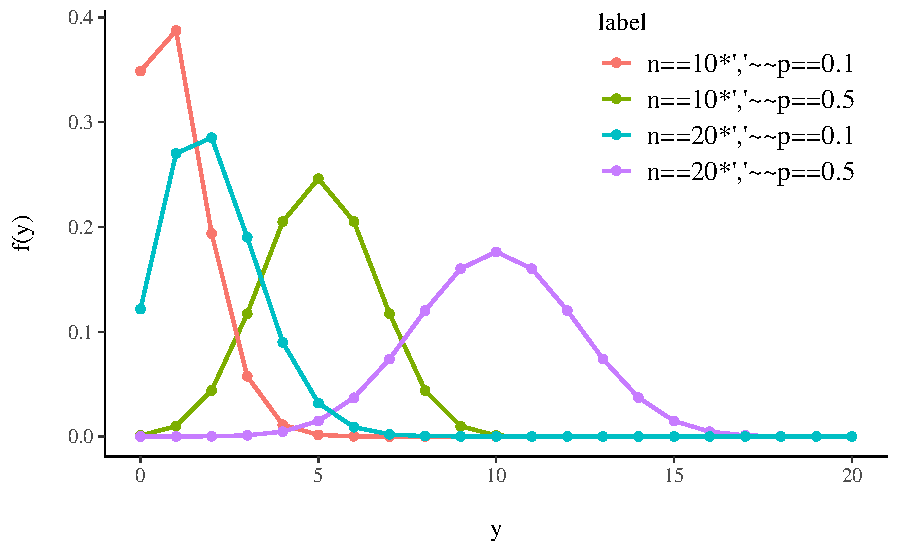
\includegraphics{022_discr_rv_distr_files/figure-latex/example-binomial-distr-1} 

}

\caption{Alcune distribuzioni binomiali. Nella figura, il parametro $\theta$ è indicato con $p$.}\label{fig:example-binomial-distr}
\end{figure}

\begin{exercise}

Usando la \eqref{eq:binomialdistribution}, si trovi la probabilità di \(y = 2\) successi in \(n = 4\) prove Bernoulliane indipendenti con \(\theta = 0.2\)

\[
\begin{aligned}
P(Y=2) &= \frac{4!}{2!(4-2)!} 0.2^{2} (1-0.2)^{4-2} \notag  \\
 &= \frac{4 \cdot 3 \cdot 2 \cdot 1}{(2 \cdot 1)(2 \cdot 1)}
0.2^{2} 0.8^{2} = 0.1536. \notag
\end{aligned}
\]

Ripetendo i calcoli per i valori \(y = 0, \dots, 4\) troviamo la distribuzione binomiale di parametri \(n = 4\) e \(\theta = 0.2\):

\begin{longtable}[]{@{}cc@{}}
\toprule
y & P(Y = y) \\
\midrule
\endhead
0 & 0.4096 \\
1 & 0.4096 \\
2 & 0.1536 \\
3 & 0.0256 \\
4 & 0.0016 \\
sum & 1.0 \\
\bottomrule
\end{longtable}

Lo stesso risultato si ottiene usando la sequente istruzione \R:

\begin{Shaded}
\begin{Highlighting}[]
\FunctionTok{dbinom}\NormalTok{(}\DecValTok{0}\SpecialCharTok{:}\DecValTok{4}\NormalTok{, }\DecValTok{4}\NormalTok{, }\FloatTok{0.2}\NormalTok{)}
\CommentTok{\#\textgreater{} [1] 0.4096 0.4096 0.1536 0.0256 0.0016}
\end{Highlighting}
\end{Shaded}

\end{exercise}

\begin{exercise}

Lanciando \(5\) volte una moneta onesta, qual è la probabilità che esca testa almeno tre volte?

In \R, la soluzione si trova con

\begin{Shaded}
\begin{Highlighting}[]
\FunctionTok{dbinom}\NormalTok{(}\DecValTok{3}\NormalTok{, }\DecValTok{5}\NormalTok{, }\FloatTok{0.5}\NormalTok{) }\SpecialCharTok{+} \FunctionTok{dbinom}\NormalTok{(}\DecValTok{4}\NormalTok{, }\DecValTok{5}\NormalTok{, }\FloatTok{0.5}\NormalTok{) }\SpecialCharTok{+} \FunctionTok{dbinom}\NormalTok{(}\DecValTok{5}\NormalTok{, }\DecValTok{5}\NormalTok{, }\FloatTok{0.5}\NormalTok{)}
\CommentTok{\#\textgreater{} [1] 0.5}
\end{Highlighting}
\end{Shaded}

Alternativamente, possiamo trovare la probabilità dell'evento complementare a quello definito dalla funzione di ripartizione calcolata mediante \texttt{pbinom()}, ovvero

\begin{Shaded}
\begin{Highlighting}[]
\DecValTok{1} \SpecialCharTok{{-}} \FunctionTok{pbinom}\NormalTok{(}\DecValTok{2}\NormalTok{, }\DecValTok{5}\NormalTok{, }\FloatTok{0.5}\NormalTok{)}
\CommentTok{\#\textgreater{} [1] 0.5}
\end{Highlighting}
\end{Shaded}

\end{exercise}

\hypertarget{valore-atteso-e-deviazione-standard}{%
\subsection{Valore atteso e deviazione standard}\label{valore-atteso-e-deviazione-standard}}

La media (numero atteso di successi in \(n\) prove) e la deviazione
standard di una distribuzione binomiale sono molto semplici:
\begin{align}
\mu    &= n\theta,  \notag \\
\sigma &= \sqrt{n\theta(1-\theta)}.
 \end{align}

\begin{proof}
Essendo \(Y\) la somma di \(n\) prove Bernoulliane indipendenti \(Y_i\), è facile vedere che
\begin{align}
\E(Y) &= \E \left( \sum_{i=1}^n Y_i \right) = \sum_{i=1}^n \E(Y_i) = n\theta, \\
\Var(Y) &= \Var \left( \sum_{i=1}^n Y_i \right) = \sum_{i=1}^n \Var(Y_i) = n \theta (1-\theta).
\end{align}
\end{proof}

\begin{exercise}
Si trovino il valore atteso e la varianza del lancio di quattro monete con probabilità di successo pari a \(\theta = 0.2\).

Il valore atteso è \(\mu = n\theta = 4 \cdot 0.2 = 0.8.\) Ciò significa che, se l'esperimento casuale venisse ripetuto infinite volte, l'esito testa verrebbe osservato un numero medio di volte pari a 0.8. La varianza è \(n \theta (1-\theta) = 4 \cdot(1 - 0.2) = 0.8\).\footnote{L'eguaglianza di \(\mu\) e \(\sigma\) è solo una peculiarità di questo esempio.}
\end{exercise}

\hypertarget{distribuzione-di-poisson}{%
\section{Distribuzione di Poisson}\label{distribuzione-di-poisson}}

La distribuzione di Poisson è una distribuzione di probabilità discreta che esprime le probabilità per il numero di eventi che si verificano successivamente ed indipendentemente in un dato intervallo di tempo, sapendo che mediamente se ne verifica un numero \(\lambda\). La distribuzione di Poisson serve dunque per contare il numero di volte in cui un evento ha luogo in un determinato intervallo di tempo. La stessa distribuzione può essere estesa anche per contare gli eventi che hanno luogo in una determinata porzione di spazio.

\begin{definition}
La distribuzione di Poisson può essere intesa come limite della distribuzione binomiale, dove la probabilità di successo \(\theta\) è pari a \(\frac{\lambda}{n}\) con \(n\) che tende a \(\infty\):
\begin{equation}
\lim_{y \rightarrow \infty} \binom{n}{y} \theta^y (1-\theta)^{n-y} = \frac{\lambda^y}{y!}e^{-\lambda}.
\end{equation}
\end{definition}

Alcune distribuzioni di Poisson sono riportate nella figura \ref{fig:examples-poisson-distrib}.

\begin{figure}[h]

{\centering 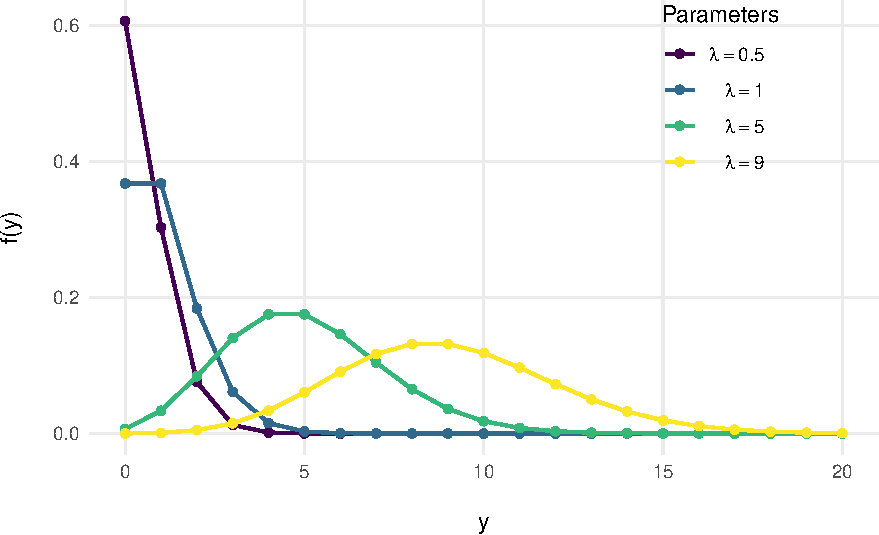
\includegraphics{022_discr_rv_distr_files/figure-latex/examples-poisson-distrib-1} 

}

\caption{Alcune distribuzioni di Poisson.}\label{fig:examples-poisson-distrib}
\end{figure}

\begin{exercise}

Supponiamo che un evento accada 300 volte all'ora e si vuole determinare la probabilità che in un minuto accadano esattamente 3 eventi.

Il numero medio di eventi in un minuto è pari a

\begin{Shaded}
\begin{Highlighting}[]
\NormalTok{lambda }\OtherTok{\textless{}{-}} \DecValTok{300} \SpecialCharTok{/} \DecValTok{60}
\NormalTok{lambda}
\CommentTok{\#\textgreater{} [1] 5}
\end{Highlighting}
\end{Shaded}

\noindent
Quindi la probabilità che in un minuto si abbiano 3 eventi è pari a

\begin{Shaded}
\begin{Highlighting}[]
\NormalTok{y }\OtherTok{\textless{}{-}} \DecValTok{3}
\NormalTok{(lambda}\SpecialCharTok{\^{}}\NormalTok{y }\SpecialCharTok{/} \FunctionTok{factorial}\NormalTok{(y)) }\SpecialCharTok{*} \FunctionTok{exp}\NormalTok{(}\SpecialCharTok{{-}}\NormalTok{lambda)}
\CommentTok{\#\textgreater{} [1] 0.14}
\end{Highlighting}
\end{Shaded}

\end{exercise}

\begin{exercise}

Per i dati dell'esempio precedente, si trovi la probabilità che un evento accada almeno 8 volte in un minuto.

La probabilità cercata è
\[
p(y \geq 8) = 1 - p (y \leq 7) = 1- \sum_{i = 0}^7 \frac{\lambda^7}{7!}e^{-\lambda},
\]
\noindent
con \(\lambda = 5\).

Svolgendo i calcoli in \R otteniamo:

\begin{Shaded}
\begin{Highlighting}[]
\DecValTok{1} \SpecialCharTok{{-}} \FunctionTok{ppois}\NormalTok{(}\AttributeTok{q =} \DecValTok{7}\NormalTok{, }\AttributeTok{lambda =} \DecValTok{5}\NormalTok{)}
\CommentTok{\#\textgreater{} [1] 0.133}
\FunctionTok{ppois}\NormalTok{(}\AttributeTok{q =} \DecValTok{7}\NormalTok{, }\AttributeTok{lambda =} \DecValTok{5}\NormalTok{, }\AttributeTok{lower.tail =} \ConstantTok{FALSE}\NormalTok{)}
\CommentTok{\#\textgreater{} [1] 0.133}
\end{Highlighting}
\end{Shaded}

\end{exercise}

\begin{exercise}

Sapendo che un evento avviene in media 6 volte al minuto, si calcoli (a) la probabilità di osservare un numero di eventi uguale o inferiore a 3 in un minuto, e (b) la probabilità di osservare esattamente 2 eventi in 30 secondi.

\begin{enumerate}
\def\labelenumi{(\alph{enumi})}
\tightlist
\item
  In questo caso \(\lambda = 6\) e la probabilità richiesta è
\end{enumerate}

\begin{Shaded}
\begin{Highlighting}[]
\FunctionTok{ppois}\NormalTok{(}\AttributeTok{q =} \DecValTok{3}\NormalTok{, }\AttributeTok{lambda =} \DecValTok{6}\NormalTok{, }\AttributeTok{lower.tail =} \ConstantTok{TRUE}\NormalTok{)}
\CommentTok{\#\textgreater{} [1] 0.151}
\end{Highlighting}
\end{Shaded}

\begin{enumerate}
\def\labelenumi{(\alph{enumi})}
\setcounter{enumi}{1}
\tightlist
\item
  In questo caso \(\lambda = 6 / 2\) e la probabilità richiesta è
\end{enumerate}

\begin{Shaded}
\begin{Highlighting}[]
\FunctionTok{dpois}\NormalTok{(}\AttributeTok{x =} \DecValTok{2}\NormalTok{, }\AttributeTok{lambda =} \DecValTok{3}\NormalTok{)}
\CommentTok{\#\textgreater{} [1] 0.224}
\end{Highlighting}
\end{Shaded}

\end{exercise}

\hypertarget{alcune-proprietuxe0-della-variabile-di-poisson}{%
\section{Alcune proprietà della variabile di Poisson}\label{alcune-proprietuxe0-della-variabile-di-poisson}}

\begin{itemize}
\item
  Il valore atteso, la moda e la varianza della variabile di Poisson sono uguali a \(\lambda\).
\item
  La somma \(Y_1 + \dots + Y_n\) di \(n\) variabili casuali indipendenti con distribuzioni di Poisson di parametri \(\lambda_{1},\dots,\lambda_{n}\) segue una distribuzione di Poisson di parametro \(\lambda = \lambda_{1}+\dots+\lambda_{n}\).
\item
  La differenze di due variabili di Poisson non è una variabile di Poisson. Basti infatti pensare che può assumere valori negativi.
\end{itemize}

\hypertarget{considerazioni-conclusive}{%
\section*{Considerazioni conclusive}\label{considerazioni-conclusive}}
\addcontentsline{toc}{section}{Considerazioni conclusive}

La distribuzione binomiale è una distribuzione di probabilità discreta che descrive il numero di successi in un processo di Bernoulli, ovvero la variabile aleatoria \(Y = Y_1 + \dots + Y_n\) che somma \(n\) variabili casuali indipendenti di uguale distribuzione di Bernoulli \(\mathcal{B}(\theta)\), ognuna delle quali può fornire due soli risultati: il successo con probabilità \(\theta\) e il fallimento con probabilità \(1 - \theta\).

La distribuzione binomiale è molto importante per le sue molte applicazioni. Nelle presenti dispense, dedicate all'analisi bayesiana, è soprattutto importante perché costituisce il fondamento del caso più semplice del cosiddetto ``aggiornamento bayesiano'', ovvero il caso Beta-Binomiale. Il modello Beta-Binomiale ci fornirà infatti un esempio paradigmatico dell'approccio bayesiano all'inferenza e sarà trattato in maniera analitica. È dunque importante che le proprietà della distribuzione binomiale risultino ben chiare.


% Bibliography
%%%%%%%%%%%%%%%%%%%%%%%%%%%%%%%%%%%%%%%%%%%%%%%%%%%%%%%%%%

\backmatter
\SmallMargins

\printbibliography
\onecolumn


% Tables (of tables, of figures)
%%%%%%%%%%%%%%%%%%%%%%%%%%%%%%%%%%%%%%%%%%%%%%%%%%%%%%%%%%


\cleardoublepage
\LargeMargins
\listoffigures


% After-body (LaTeX code inclusion)
%%%%%%%%%%%%%%%%%%%%%%%%%%%%%%%%%%%%%%%%%%%%%%%%%%%%%%%%%%




% Back cover
%%%%%%%%%%%%%%%%%%%%%%%%%%%%%%%%%%%%%%%%%%%%%%%%%%%%%%%%%%%

% Even page, small margins, no running head, no page number.
\evenpage
\SmallMargins
\thispagestyle{empty}

\begin{normalsize}

\begin{description}

\selectlanguage{italian}
\item[Abstract]
This document contains the material of the lessons of Psicometria B000286 (2021/2022) aimed at students of the first year of the Degree Course in Psychological Sciences and Techniques of the University of Florence, Italy.
\item[Keywords]
Data science, Bayesian statistics.
~\\

\end{description}

\end{normalsize}


\end{document}
